\documentclass{article}
\usepackage{natbib}
%\setcitestyle{aysep={}}
\usepackage[labelfont=bf]{caption}
\usepackage{subcaption}
\usepackage{graphicx}
\usepackage{float}
%\bibliographystyle{apalike}
%\bibliographystyle{agsm}
\bibliographystyle{groundwater}
\usepackage{lineno}
\linenumbers

\usepackage{geometry}
\geometry{letterpaper}
\geometry{margin=1in}

\usepackage{setspace}
\doublespacing
\captionsetup[figure]{font={stretch=2}}
\usepackage[nomarkers,figuresonly]{endfloat}
\usepackage[nottoc]{tocbibind}

\usepackage{authblk}
\usepackage{xcolor}
\usepackage{ulem}

\newcommand{\matr}[1]{\mathbf{#1}}
\renewcommand{\bibname}{References}

\title{Accurate Simulation of Flow through Dipping Aquifers with MODFLOW 6 Using Enhanced Cell Connectivity}

\author{
	Alden M. Provost (corresponding author), U.S. Geological Survey, Integrated Modeling and Prediction Division, U.S. Geological Survey, 12201 Sunrise Valley Dr, Reston, VA, USA; aprovost@usgs.gov \\
	\and 
	Kerry Bardot, School of Earth Sciences, University of Western Australia, Perth, Australia; kerry.bardot@research.uwa.edu.au \\
	\and 
	Christian D. Langevin, U.S. Geological Survey, Integrated Modeling and Prediction Division, 2280 Woodale Drive, Mounds View, MN, USA; langevin@usgs.gov \\
	\and 
	James L. McCallum, School of Earth Sciences, University of Western Australia, Perth, Australia; james.mccallum@uwa.edu.au \\
	}


\date{\today}

\begin{document}

\noindent Methods Brief/

%\maketitle
{\let\newpage\relax\maketitle}

\textbf{Conflict of interest:} None.

\textbf{Key words:} groundwater flow simulation, discretization, vertically offset grid, dipping layers, cell connectivity, multi-point flux approximation, sedimentary structures

\textbf{Article impact statement:} Accurate simulation of groundwater flow through dipping aquifers using MODFLOW 6 can require enhanced cell connectivity and use of a multi-point formulation for flow between cells. This can be achieved using an unstructured grid and the XT3D flow formulation.

\begin{abstract}

In simulations of groundwater flow through dipping aquifers, layers of model cells are often ``deformed'' to follow the top and bottom elevations of the aquifers. When this approach is used in MODFLOW, adjacent cells within the same model layer are vertically offset from one another, and the standard conductance-based (two-point) formulation for flow between cells does not rigorously account for these offsets. The XT3D multi-point flow formulation in MODFLOW 6 is designed to account for geometric irregularities in the grid, including vertical offsets, and to provide accurate results for both isotropic and anisotropic groundwater flow.  A recent study evaluated the performance of the standard formulation and XT3D using a simple, synthetic benchmark model of a steeply dipping aquifer. Although XT3D generally improved the accuracy of flow simulations relative to the standard formulation as expected, neither formulation produced accurate flows in cases that involved large vertical offsets. In this paper, we explain that the inability of XT3D to produce accurate flows in the steeply dipping aquifer benchmark was not due to an inherent limitation of the flow formulation, but rather to the limited cell connectivity inherent in the most commonly used discretization packages in MODFLOW 6. Furthermore, we demonstrate that XT3D is able to produce the expected accuracy when adequate cell connectivity is introduced using MODFLOW's unstructured grid type and the aquifer is discretized vertically using at least two model layers.

\end{abstract}

\section*{Introduction}

Numerical simulation of layered aquifer systems can involve a tradeoff between efficiency and accuracy. A traditional approach to discretizing layered aquifer systems, called the ``grid overlay'' method by \cite{hoaglund2003}, maps the heterogeneous hydrologic properties onto a rectilinear grid \citep{modflow84}. Although this method preserves the benefits of the rectilinear grid structure, it can require a large number of model grid layers to adequately discretize hydrogeologic layers of variable dip and thickness \citep{Zyvoloski2006}.

An alternative approach, called the ``boundary-matching" method by \cite{hoaglund2003}, allows model grid layers to "deform" vertically to follow the undulations of hydrogeologic layers. This commonly used method ``minimize[s] the number of model [grid] layers required to simulate an aquifer system'' \citep{modflow84}. However, the non-orthogonality of the resulting grid can be a source of substantial model error \citep{hoaglund2003}.

In models based on the Control Volume Finite Difference (CVFD) method, which is the method used in the MODFLOW family of hydrologic simulation codes \citep{modflow6gwf, langevin2024}, the loss of accuracy associated with the boundary-matching approach results from the use of a "two-point" formulation to calculate flows between adjacent grid cells. In the two-point formulation, the flow between two cells is proportional to the difference between the heads calculated in those two cells. For simulations of flow through isotropic porous media, the two-point flow formulation is most accurate when the grid satisfies the so-called ``CVFD requirement" \citep{modflowusg, modflow6gwf} that the straight-line connection between two cell centers must intersect the midpoint of the cell interface at a right angle \citep{narasimhan1976integrated}. However, boundary-matching grids violate the CVFD requirement at vertical interfaces between cells in the same model layer because the corresponding cell connections are not strictly horizontal.

In MODFLOW, the top and bottom surfaces of model cells are horizontal \citep{modflow6gwf}. Thus, when boundary matching is implemented in a two-dimensional (2D) cross-sectional or three-dimensional (3D) MODFLOW model, the tops of laterally adjacent cells are vertically offset from each other (as are the cell bottoms) and can follow the undulations of the aquifer boundaries only on average. Following \cite{bardot2023}, we call this type of grid ``vertically offset." In a vertically offset grid, subhorizontal cell connections across vertical cell interfaces violate the CVFD requirement, which reduces the accuracy of two-point flow formulation. For an isotropic aquifer, \cite{hoaglund2003} note that ``the error range is smaller for smaller dips, generally $<20$\% within $10^{\circ}$ of dip."

The introduction of unstructured grids into MODFLOW \citep{modflowusg, modflow6gwf} presented new ways for a grid to violate the CVFD requirements. To help overcome the limitations of the two-point flow formulation on geometrically irregular grids, MODFLOW-USG and MODFLOW 6 offer a Ghost-Node Correction (GNC) Package \citep{modflowusg, modflow6gwf}. However, configuration of optimal ghost node locations and interpolation weights is problem-dependent, and we are not aware of guidelines for handling general unstructured grids or arbitrarily oriented 3D anisotropy.

The optional XT3D flow formulation \citep{modflow6xt3d} in MODFLOW 6 offers a more ``automatic" alternative to ghost nodes. XT3D is a multi-point flow formulation \citep{edwards1998, aavatsmark2002} based on gradient reconstruction \citep{mavriplis2003leastsq, diskin2008accuracy}. By performing flow calculations using Darcy's Law in its tensorial form using a multi-point approximation of the head gradient vector, XT3D accounts for both arbitrarily oriented anisotropy and geometric irregularity of the grid. In theory, XT3D should be able to compensate for the geometric irregularity introduced by vertical offsets between adjacent cells in the same grid layer.

\cite{bardot2023} tested the ability of MODFLOW 6 to accurately simulate flow through sedimentary structures, both with and without XT3D. The simplest 2D cross-sectional (``transect") version of their benchmark model simulated flow through a steeply dipping, homogeneous, isotropic aquifer of uniform thickness embedded between two confining units. In test runs that used the boundary-matching method on a vertically offset grid, both the two-point flow formulation and XT3D produced flows that differed markedly from the expected magnitude and direction throughout the aquifer, regardless of how finely the aquifer was discretized both vertically and horizontally. They noted, however, that a preliminary analysis by two authors of the present work (Provost and Langevin) suggested that the limited cell connectivity offered by the layered, vertically offset grids was inadequate to allow an accurate flow solution.

To our knowledge, the implications of limited cell connectivity in layered, vertically offset grids for the accuracy of simulated flows, and the potential to improve accuracy using enhanced connectivity between model layers, have not been previously recognized or investigated. In this paper, we present theoretical explanations for why ``layered" connectivity in a vertically offset grid is inadequate for accurate simulation of flows in steeply dipping hydrogeologic layers, and why using what we call ``full" cell connectivity together with XT3D should improve accuracy. Then, in a set of test problems similar to those of \cite{bardot2023}, we demonstrate the effectiveness of using full connectivity with XT3D. Finally, we discuss the implications of our findings for practical groundwater problems involving steeply dipping hydrogeologic layers.

\section*{Theory}

Versions of MODFLOW prior to MODFLOW-USG \citep{modflowusg} supported only structured grids composed of rows, columns, and layers of cells, which could be vertically offset. This grid type, called ``DIS," continues to be supported in MODFLOW-USG and MODFLOW 6, which also offer an unstructured grid type called ``DISU" \citep{modflowusg, modflow6gwf}. In addition, MODFLOW 6 offers an  unstructured grid type called ``DISV," which is based on specification of cell vertices \citep{modflow6gwf}. The DIS and DISV grid types are based on model layers, with the same horizontal grid structure within each layer. In a DIS or DISV grid, a connection between two cells in different model layers is created automatically if and only if one cell is directly below the other and neither cell has been optionally excluded from the model domain by the user. The DISU grid type is more flexible and, in MODFLOW 6, does not require the grid to have a layered structure. (The DISU grid type in MODFLOW-USG is similarly flexible but retains the concept of layers.) In a DISU grid, the user explicitly specifies all connections between grid cells. Thus, when used to represent a grid with a layered structure, as in this work, the DISU grid type allows connections to exist between any two cells, whether they are in the same layer or different layers. Grid geometry and connectivity information supplied by the discretization package (DIS, DISV, or DISU) is used by the MODFLOW 6 Node Property Flow (NPF) Package to formulate expressions for groundwater flow between cells in terms of heads calculated at cell centers. By default, the NPF Package uses a two-point flow formulation, which we call the ``conductance-based'' formulation. The optional, multi-point XT3D flow formulation can be activated simply by including the corresponding keyword in the NPF Package input.

\begin{figure}
	\begin{center}
	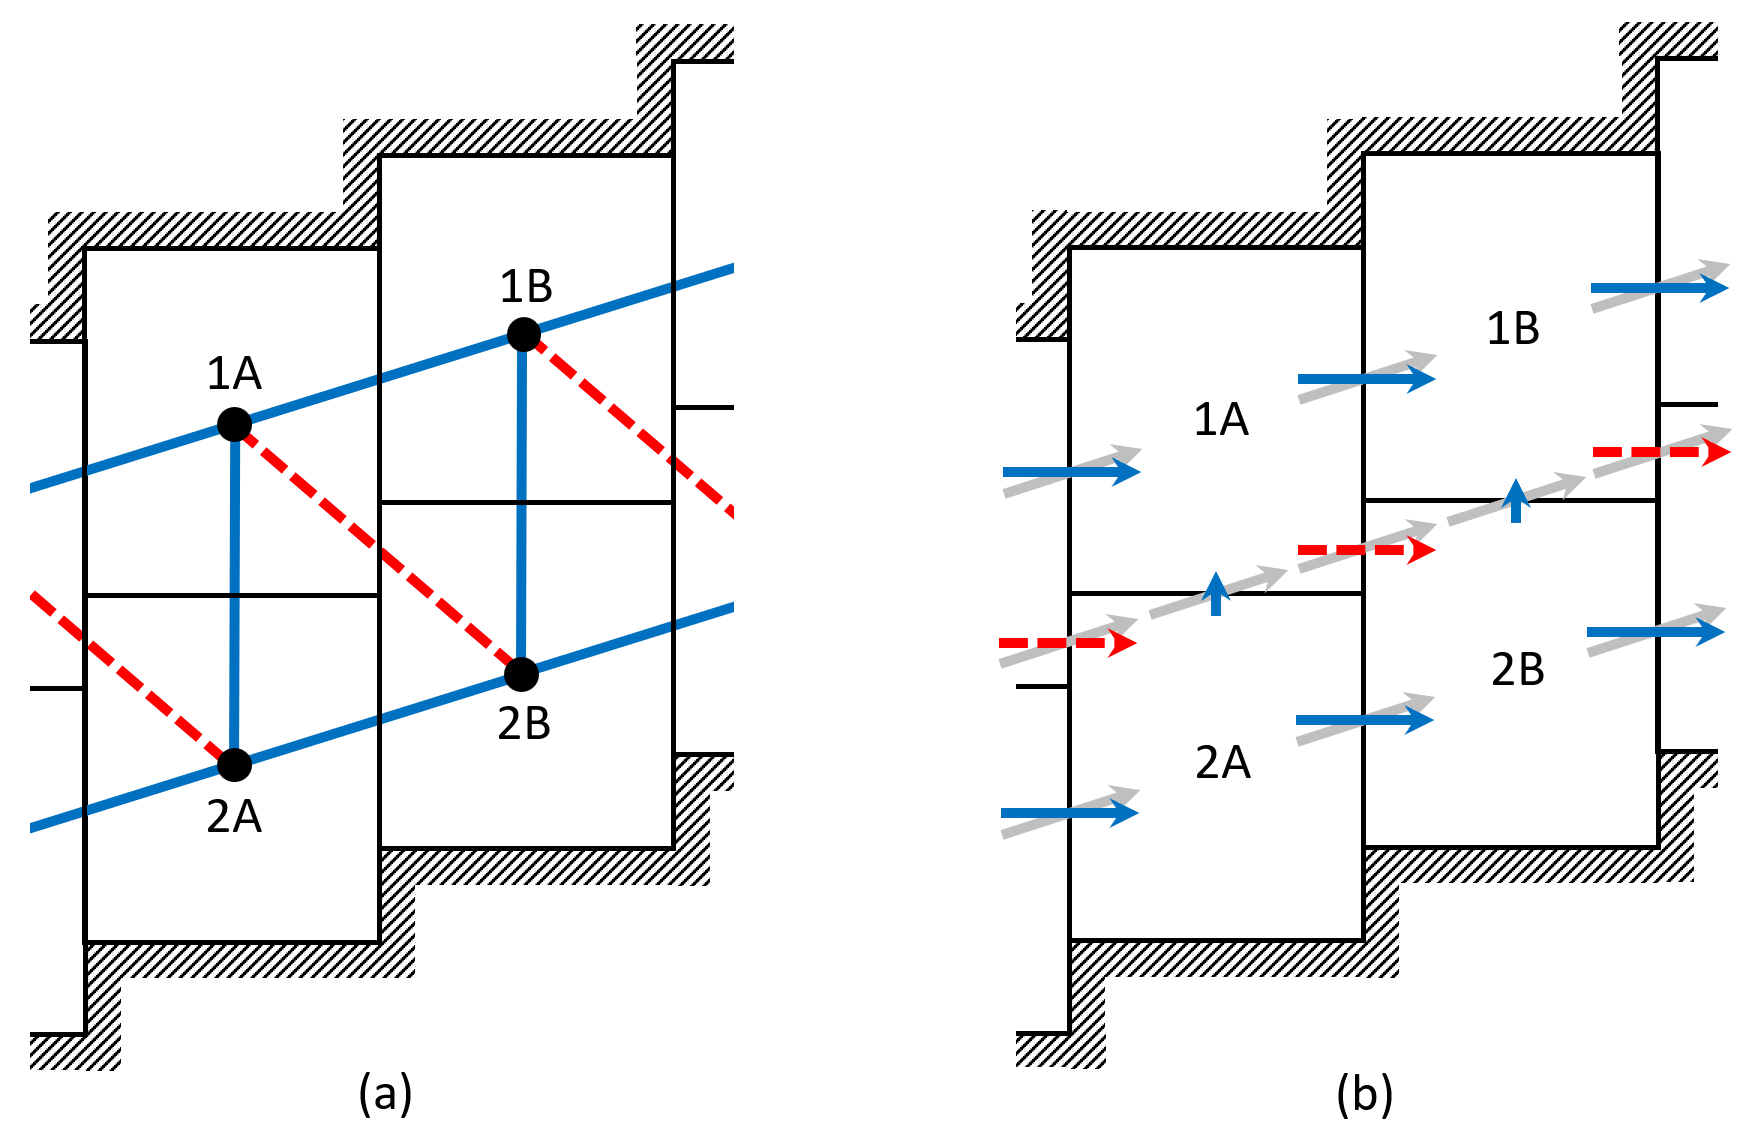
\includegraphics[scale=1.0]{../figures/fig1_paper.png}
	\caption{Schematics showing (a) cell connectivity and (b) cell-cell interface fluxes in a two-grid-layer model of a dipping hydrogeologic layer. Hatching denotes impermeable boundaries along the top and bottom of the hydrogeologic layer. In (a), black circles represent cell centers. Solid blue lines represent hydraulic connections between cells in a layered-connectivity grid. Dashed red lines represent additional connections that must be made to achieve full connectivity. In (b), solid gray arrows represent the uniform groundwater flux the model is attempting to simulate. Solid blue arrows represent components of the uniform groundwater flux normal to the horizontal and vertical cell-cell interfaces in the layered-connectivity grid. Dashed red arrows represent components of the uniform groundwater flux normal to the additional vertical cell-cell interfaces introduced to represent the full connectivity.}
	\label{fig:schem-conn-area-flux}
	\end{center}
\end{figure}

Figure \ref{fig:schem-conn-area-flux}a illustrates what we refer to as "layered" and "full" cell connectivity. The focus is on a group of four cells in a two-grid-layer, vertically offset MODFLOW 6 model of fully saturated flow through a permeable hydrogeologic layer (aquifer) with impermeable top and bottom boundaries. If the grid is represented using a layered grid type (DIS or DISV), the grid has what we call ``layered connectivity": a cell is hydraulically connected to each laterally adjacent cell in the same grid layer (regardless of whether or not the cell faces actually overlap), and with each overlying and underlying cell, as indicated by the solid blue lines that connect cell centers in Figure \ref{fig:schem-conn-area-flux}a. In layered connectivity, two cells that have overlapping vertical faces but are in different grid layers (e.g., cells 1A and 2B) notably do not have a direct hydraulic connection. The addition of such connections between cells in different grid layers, as indicated by the dashed red lines that connect cell centers in Figure \ref{fig:schem-conn-area-flux}a, results in a grid with what we call ``full connectivity.''  Implementation of full connectivity in the current version of MODFLOW 6 \citep{modflow650software} requires that the vertically offset grid be represented using the fully unstructured (DISU) grid type.

The need for full cell connectivity to accurately simulate flow along the dipping hydrogeologic layer is illustrated in Figure \ref{fig:schem-conn-area-flux}b. Components of the groundwater flux (specific discharge) vector are displayed on each cell-cell interface and are representative of steady, uniform flow along the hydrogeologic layer. Gray vectors represent the uniform flux oriented along the hydrogeologic layer, which the model is attempting to simulate. Solid blue vectors represent the flux components normal to cell-cell interfaces that correspond to solid blue connections in Figure \ref{fig:schem-conn-area-flux}a, which are common to both the layered-connectivity and full-connectivity grids. Dashed red vectors represent the flux components normal to cell-cell interfaces that correspond to dashed red connections in Figure \ref{fig:schem-conn-area-flux}a, which are lacking in the layered-connectivity grid.

The solid blue vectors in Figure \ref{fig:schem-conn-area-flux}b show that to simulate steady, uniform flow along the dipping hydrogeologic layer, cells must exchange water not only ``horizontally'' with neighboring cells in the same grid layer, but also vertically with cells in the adjacent grid layer. Specifically, there must be flow from cells in the lower grid layer to cells in the upper grid layer, which corresponds to the vertical component of the groundwater flux. Note, however, that the solid blue vectors alone are incompatible with steady, uniform flow along the hydrogeologic layer because the exchange of water between the two grid layers is in one direction only: upward. Such a steady-state flow configuration would imply continuous depletion of flow within the lower grid layer and accumulation of flow within the upper grid layer as one moves along the hydrogeologic layer in the direction of flow. Thus, the steady, uniform flow represented by the gray vectors cannot be simulated accurately without some mechanism for returning flow from the upper grid layer to the lower grid layer. The full-connectivity grid provides such a mechanism by offering additional connections between cells in adjacent grid layers. Vertical flows from the lower grid layer to the upper grid layer, represented by vertical solid blue vectors in Figure \ref{fig:schem-conn-area-flux}b, can be returned to the lower grid layer by nominally ``horizontal'' flows, represented by dashed red vectors in Figure \ref{fig:schem-conn-area-flux}b. Although this concept has been illustrated using a two-grid-layer model for simplicity, the same reasoning applies given any number of grid layers.

Vertically offset grids violate the CFVD requirement because nominally ``horizontal'' connections between cell centers in the same grid layer are not strictly horizontal and therefore not perpendicular to the vertical cell-cell interfaces they intersect. For example, in Figure \ref{fig:schem-conn-area-flux}a, the connection between cells 1A and 1B is not perpendicular to the cell-cell interface, which reduces the accuracy of the conductance-based formulation.

Once the full connectivity is established, it is the role of the flow formulation to account properly for the geometry of the grid, a task for which XT3D was specifically designed. However, XT3D alone cannot compensate for cell connectivity that does not provide adequate pathways for flow. This explains why using XT3D did not improve the simulation results substantially on the layered-connectivity grid in the benchmark tests of \cite{bardot2023}.  In the middle section of the hydrogeologic layer, away from the end boundary conditions, the flow solution approached steady, uniform flow the only way that it could given the limited connectivity: by suppressing vertical flows between grid layers, thereby rendering the overall flow approximately horizontal.

The arguments presented in this section suggest that, in addition to the use of XT3D, full connectivity can be important for obtaining an accurate flow solution in MODFLOW 6 simulations that involve steeply dipping hydrogeologic layers. The next section presents results of simulations designed to test this hypothesis.

\section*{Description of Test Problem}

The test problem is patterned after the cross-sectional (transect) benchmark of \cite{bardot2023}. It attempts to simulate uniform flow in an inclined permeable hydrogeologic layer (``aquifer'') embedded in less permeable material (the ``domain'').

To simulate flow along an aquifer of uniform thickness inclined at angle $\theta$ relative to the horizontal ($30^{\circ}$ for the base case), heads are specified at the centers of cells along the perimeter of the model using a formula that corresponds to a uniform, unit head gradient:
\begin{equation}
\label{eqn:head_analyt_along}
h = - x \cos \theta - z \sin \theta,
\end{equation}

\noindent where $h$ is head in meters and $x$ and $z$ are the horizontal and vertical model coordinates, respectively, in meters. The hydraulic conductivity of the aquifer is set to 1 m/d (meter per day) so that the analytical flow solution is a groundwater flux of 1 m/d along the aquifer. In the base case, the conductivity of the domain surrounding the aquifer is set to $10^{-6}$ m/d to effectively isolate the aquifer hydraulically.

The test simulations use grids of MODFLOW 6 DISU (unstructured) type, which offers the flexibility to implement either layered or full connectivity. In all cases, a grid of MODFLOW 6 DIS (structured) type is first created and then converted to a DISU grid. In simulations that use layered connectivity, the DISU grid is formulated to have the same cell geometry and connectivity as the original DIS grid. In simulations that use full connectivity, additional connections between adjacent layers are added during the conversion process. The base case uses grids consisting of 11 columns and 9 layers of cells, with 3 layers within the aquifer, 3 layers in the domain above the aquifer, and 3 layers in the domain below the aquifer.  The model is 11 m wide, and each column is 1 m wide. Cells within the aquifer are square (1 m x 1 m). Corner cells in the lower left and upper right corner were also set to be the same dimension as the aquifer cells. The resulting base model vertical height is 14.77 m.  

The above description represents the base-case test problem. However, the results also include simulations designed to investigate the effects of varying the gridding resolution, the dip angle of the aquifer, the conductivity contrast between the aquifer and the domain, and the anisotropy of the conductivity tensor.

A link to the Jupyter notebooks and MODFLOW version 6.5.0 executable code used to create and run the test problem is available in the Supporting Information section. The notebooks leverage the capabilities of FloPy \citep{bakker2016scripting, hughes2024flopy} to assist in setting up input for and processing results from the MODFLOW 6 simulations. A Python script for converting structured, DIS grids to unstructured, DISU grids with full connectivity is included.

\section*{Results and Discussion}

To demonstrate the effect of cell connectivity on the accuracy of simulated flow through a steeply dipping aquifer, results for the base case described in the previous section are compared for simulations that use either layered or full connectivity, and either the standard conductance-based (two-point) flow formulation or the XT3D (multi-point) flow formulation. The base case is then modified to investigate the effects of grid resolution, aquifer dip angle, conductivity contrast between the aquifer and the surrounding domain, and anisotropic hydraulic conductivity.

Plots of specific discharge (groundwater flux) at cell centers and flows across cell-cell interfaces (face flows) calculated by MODFLOW 6 are used to illustrate the accuracy of the simulated flows. The magnitude and direction of specific discharge at the cell in the center of the aquifer, at which boundary effects are presumably minimized, and the total volumetric flow rate entering the aquifer through the left-hand boundary, which consists of constant-head (CHD) cells, are also reported as representative values of flow. Maximum head errors are also reported for the base case.

Specific discharge at cell centers is calculated in a postprocessing step using distance-weighted interpolation of face flows calculated by MODFLOW 6 and reported in the binary budget output file. For the purpose of illustrating and evaluating the results of this idealized benchmark, specific discharge in cells within the aquifer is calculated using only face flows between cells within the aquifer. Likewise, specific discharge in cells within the surrounding domain is calculated using only face flows between cells within the domain. These specific discharge values are different from those reported in the binary budget output file by MODFLOW 6 because MODFLOW interpolates specific discharge in a cell using all of the face flows for that cell, including flows across cell faces on the aquifer-domain boundary. The flows reported by MODFLOW represent an ``average'' of the different flows on either side of the aquifer-domain boundary. Therefore, specific discharge calculated in a cell adjacent to the aquifer-domain boundary is affected by the different flow rate on the other side of the boundary. Although this is an unavoidable consequence of vertically offset discretization in practical applications, and not necessarily a problem, users should be aware of these effects when interpreting the results of MODFLOW 6 dispersive-transport and MODPATH particle-tracking simulations.

\subsection*{Effects of Cell Connectivity and Flow Formulation}

The results shown in Figures \ref{fig:fig2}a and b, which are based on a vertically offset grid with layered connectivity, are consistent with the findings of \cite{bardot2023}. Despite boundary heads designed to induce specific discharge of 1 m/d along the $30^{\circ}$ incline of the aquifer, the simulated flow within the aquifer is predominantly horizontal, and the magnitude of the specific discharge at the center of the aquifer (``flux magnitude'') and the total flow entering the aquifer are overestimated by approximately 15\% and 18\%, respectively. The XT3D flow formulation is unable to compensate for the inadequate cell connectivity (Figure \ref{fig:fig2}b), which does not allow flow between laterally adjacent cells in different grid layers.

The vertically offset grid with full connectivity (Figures \ref{fig:fig2}c and d) shows substantially improved results, even for the standard flow formulation (Figure \ref{fig:fig2}c), which overestimates the flux magnitude and total flow by approximately 3\% and 9\%, respectively. Using the XT3D flow formulation provides the most accurate results, as expected (Figure \ref{fig:fig2}d), reducing the errors in flux magnitude and total flow to approximately $-2 \times 10^{-4}$\% and $2 \times 10^{-4}$\%, respectively.

\begin{figure}[p!]
	\begin{center}
	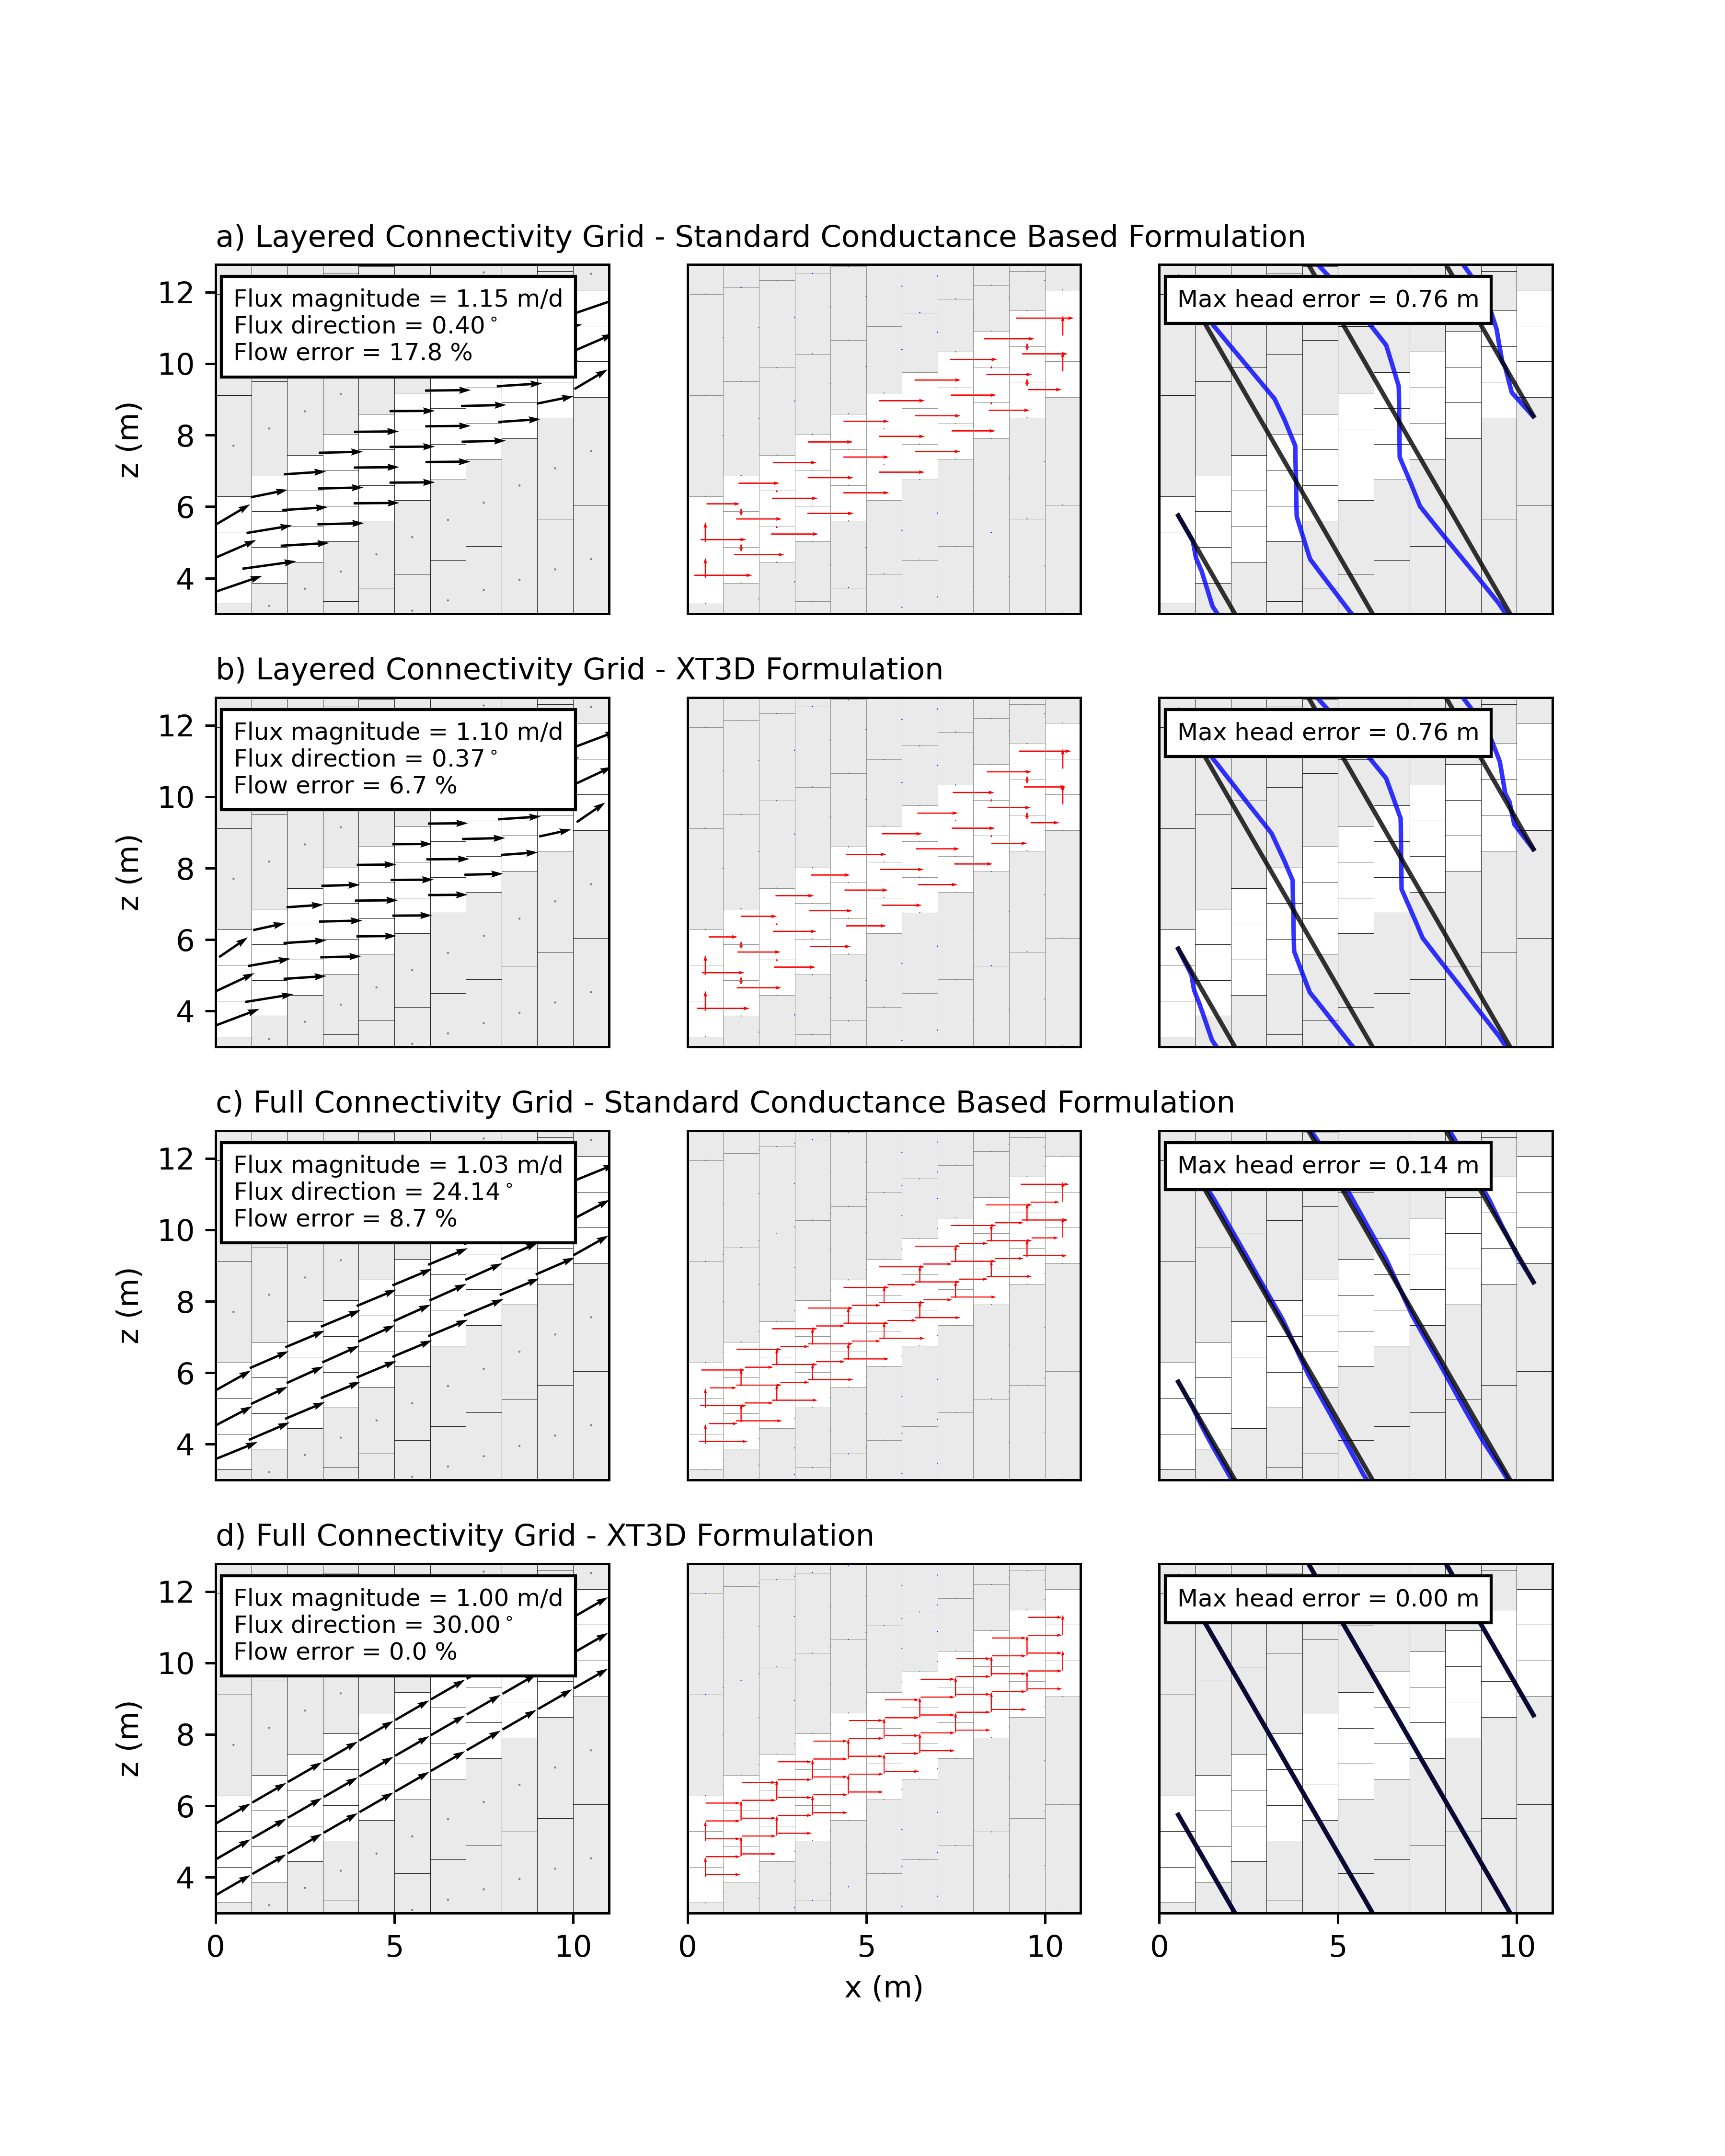
\includegraphics[scale=0.75]{../figures/fig2_paper.png}
	\caption{Numerical results for the test problem using base-case settings for layered-connectivity and full-connectivity grids, with the standard conductance-based formulation as well as the XT3D formulation. The left panel of each scenario shows the calculated specific discharge at each cell center (arrows). The middle panel shows the face flows (arrows). The right panel shows head contours for the analytical solution (dashed black) as well as the numerical solution (solid blue). Flux magnitudes, flux directions (angles), and head errors are reported to two decimal places. Percent errors in flow are reported to one decimal place.}
	\label{fig:fig2}
	\end{center}
\end{figure}

\subsection*{Effects of Grid Resolution}

\begin{figure}
	\begin{center}
	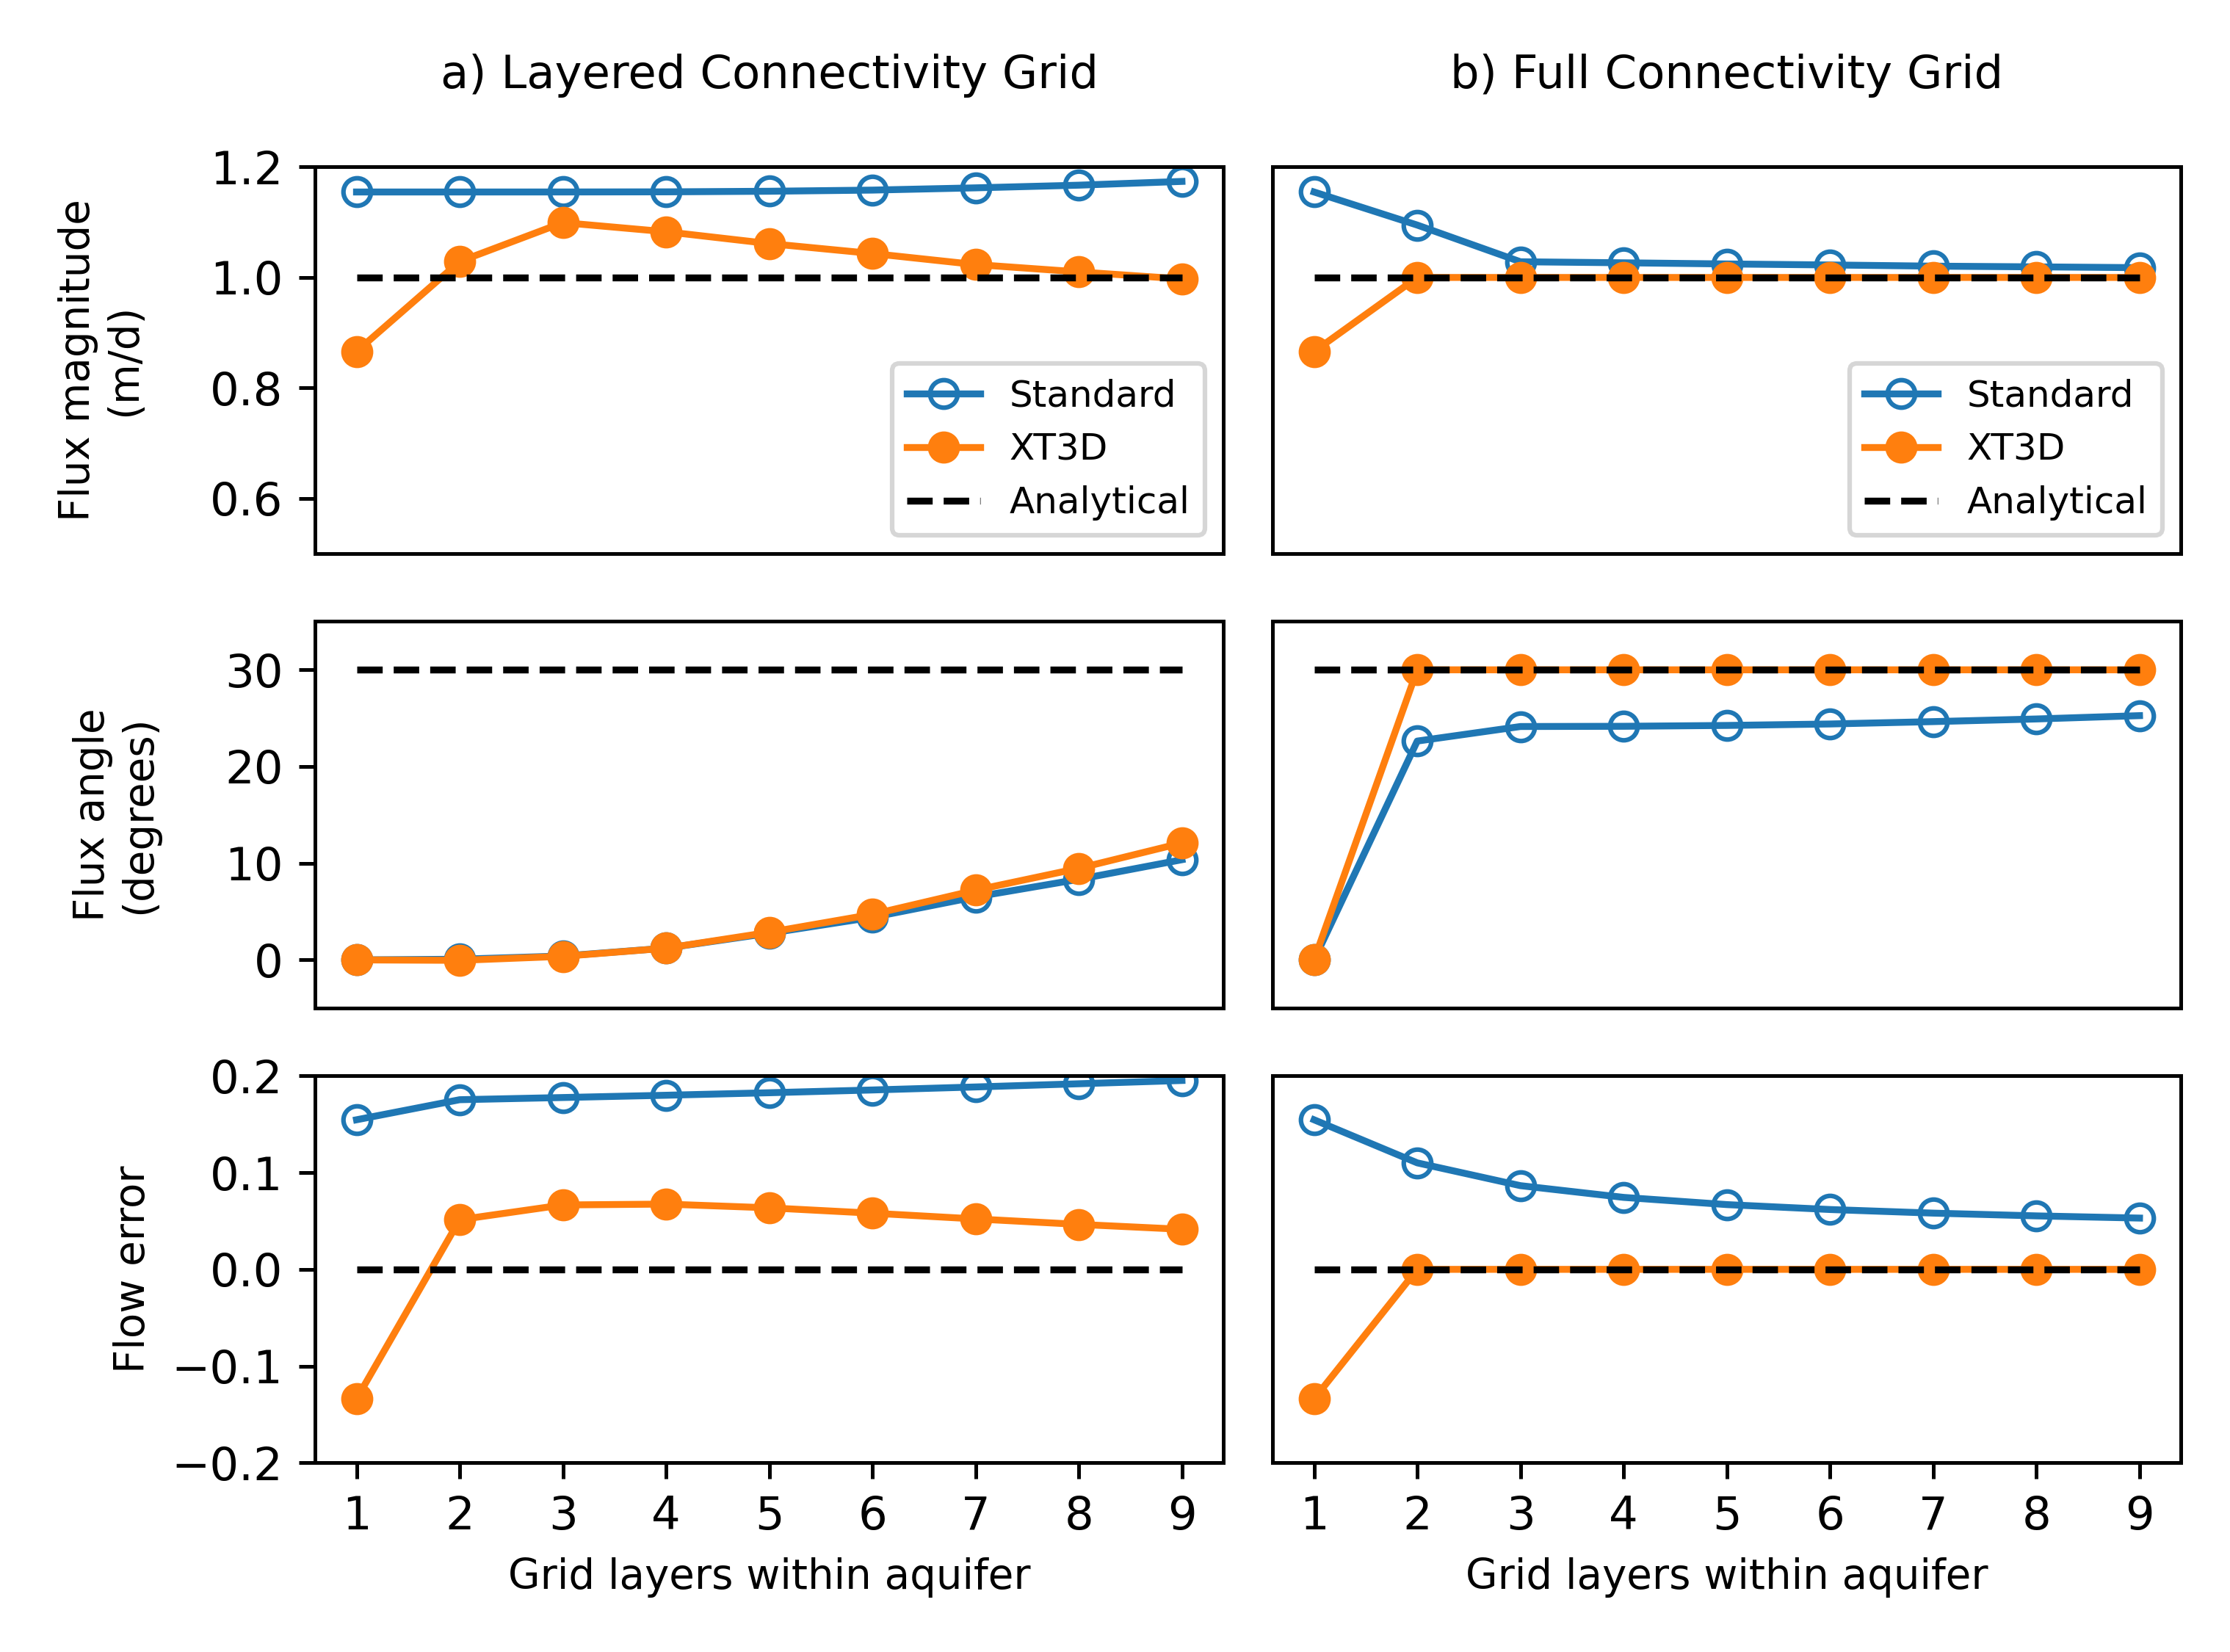
\includegraphics[scale=0.9]{../figures/fig3_paper.png}
	\caption{Graphs indicating how the number of grid layers within the aquifer affects the flux magnitude in the center cell (top), the flux direction in center cell (middle) and the volumetric flow through the aquifer (bottom). Errors are minimized by using full connectivity (right column), the XT3D flow formulation (orange lines with solid circles) and at least two grids layers in the aquifer.}
	\label{fig:fig3}
	\end{center}
\end{figure}

Groundwater models often use layered-connectivity grids \citep{Reilly2004}. Although the practice is less common today than it once was, models are sometimes configured using one grid layer per hydrogeologic unit. The simulations in this subsection investigate the effect of vertically discretizing the aquifer using multiple grid layers (Figure \ref{fig:fig3}). The base case uses three grid layers to represent the aquifer. When the number of grid layers is altered, the horizontal discretization is also adjusted to maintain square cells inside the aquifer, thus, maintaining a constant cell aspect ratio. We compare the simulated flux magnitude and direction in the cell at the center of the aquifer, as well as volumetric flow through the aquifer, against the analytical solution.

The results in Figure \ref{fig:fig3} confirm that the use of full connectivity and the XT3D flow formulation reduces the errors in calculated flows, provided at least two grid layers are used to vertically discretize the aquifer. For example, when the aquifer is represented using two layers with layered connectivity, the flow error is approximately 18\% and 5\% for the standard and XT3D flow formulations, respectively. Use of full connectivity reduces these errors to approximately 11\% and $3 \times 10^{-4}$\%, respectively. When a single grid layer is used to represent the aquifer, the enhanced connectivity needed to achieve an accurate solution is not possible, and the XT3D flow formulation is unable to compensate for the inadequate connectivity. With full connectivity and the XT3D flow formulation, using more than two layers to discretize the aquifer provides no substantial benefit in our benchmark problem (Figure \ref{fig:fig3}b).

\subsection*{Effects of Dip Angle and Conductivity Contrast}

The base case uses an aquifer dip angle of 30$^{\circ}$ and a conductivity contrast between domain and aquifer of $10^{-6}$:1. In this subsection, we investigate the behavior of the flow solution for aquifer dip angles ranging from 0 to 80$^{\circ}$. We also examine the behavior for a range of conductivity contrasts by setting the domain conductivity equal to and to 1/2, 1/5, 1/10 and 1/100 that of the aquifer. Simulated flux magnitude and direction at the center cell for all combinations are plotted against the analytical solution in Figure \ref{fig:fig4}. 

With layered connectivity and the standard conductance-based flow formulation (Figure \ref{fig:fig4}a), the magnitude of the error in the flux magnitude (left panel) is similar for all of the conductivity ratios simulated and increases with increasing aquifer dip angle. The magnitude of the error in the flux direction (right panel) increases with decreasing ratio of domain conductivity to aquifer conductivity (increasing conductivity contrast). As the surrounding domain becomes much less conductive than the aquifer, the flow direction tends toward horizontal, as shown by the ``flattening'' of the curve toward a flux direction of zero degrees as the conductivity ratio decreases from 1.0 to 0.01 in Figure \ref{fig:fig4}a.

With layered connectivity and the XT3D flow formulation (Figure \ref{fig:fig4}b), the magnitude of the error in the flux magnitude (left panel) increases with decreasing conductivity ratio and increasing aquifer dip angle. The magnitude of the error in the flux direction (right panel) increases with decreasing conductivity ratio. As the surrounding domain becomes much less conductive than the aquifer, the flow direction tends toward horizontal in Figure \ref{fig:fig4}b, as occurs with the standard flow formulation in Figure \ref{fig:fig4}a.

With full connectivity and the standard conductance-based flow formulation (Figure \ref{fig:fig4}c), the maximum error in the flux magnitude is less than 17\% of the analytical solution of 1 m/d and the maximum error in the flux direction is less than 10$^{\circ}$ at dip angles less than 40$^{\circ}$ for all of the conductivity ratios simulated. At a dip angle of  45$^{\circ}$, cells that are nominally in the same grid layer within the aquifer no longer share any interfacial area, thus becoming hydraulically disconnected from one another. A second transition in connectivity occurs at a dip angle of approximately 63$^{\circ}$, and at a dip angle of approximately 72$^{\circ}$ the vertical columns of cells within the aquifer are completely disconnected from their neighbors to either side. When the discretization used to represent the aquifer becomes substantially disconnected, it cannot be expected to support accurate results. Note that in our benchmark problem the cells within the aquifer are square. For the same vertical discretization but coarser horizontal discretization, transitions in connectivity within the aquifer would occur at smaller dip angles due to the smaller vertical-to-horizontal aspect ratio of the cells.

With full connectivity and the XT3D flow formulation (Figure \ref{fig:fig4}d), the maximum error in the flux magnitude is less than 3\% of the analytical solution of 1 m/d and the maximum error in the flux direction is less than 1$^{\circ}$ at dip angles less than 40$^{\circ}$ for all of the conductivity ratios simulated. The effects of hydraulic disconnection of cells on errors in flow magnitude and flow direction are evident at approximately 63$^{\circ}$ and 45$^{\circ}$, respectively. Overall, use of full connectivity with the XT3D flow formulation substantially reduces the error in calculated flows.

\begin{figure}[p!]
\centering
\begin{subfigure}{0.9\textwidth}
	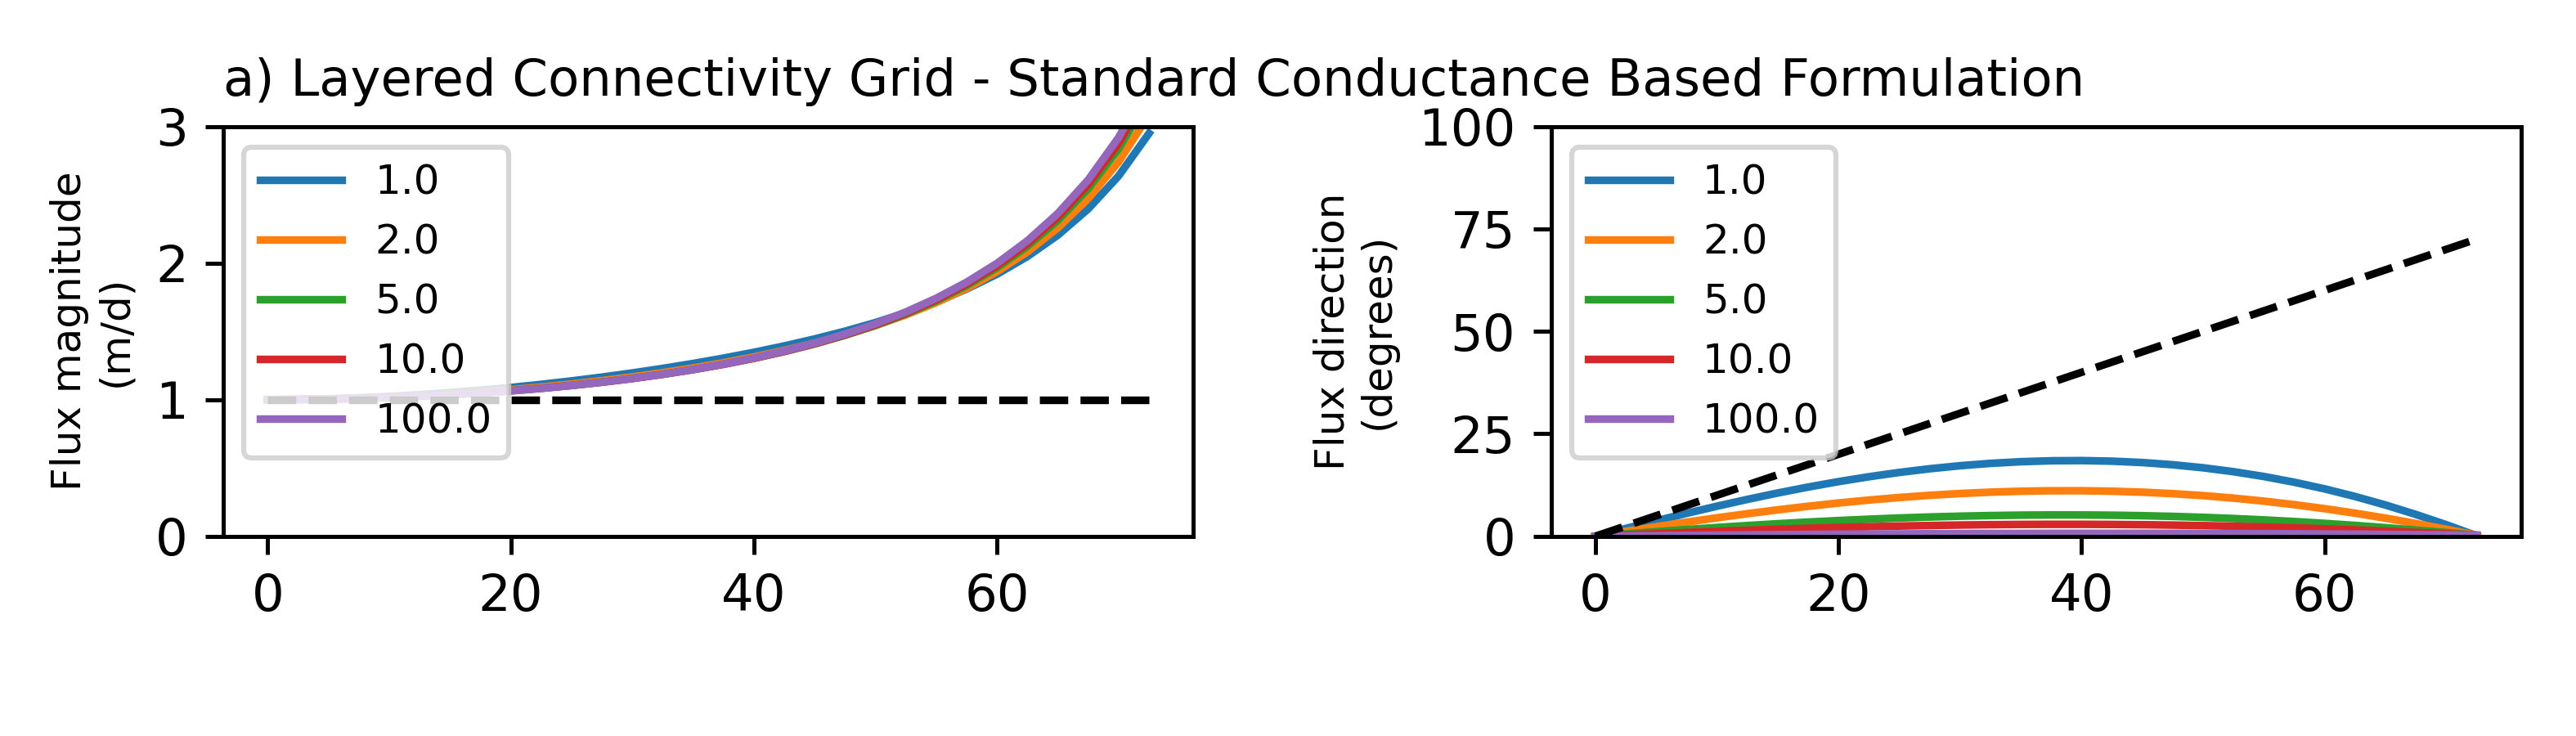
\includegraphics[width=\textwidth]{../figures/fig4_0_paper.png}
%	\caption{layered-connectivity grid, standard conductance-based formulation}
%	\label{fig:fig4a}
\end{subfigure}
\begin{subfigure}{0.9\textwidth}
	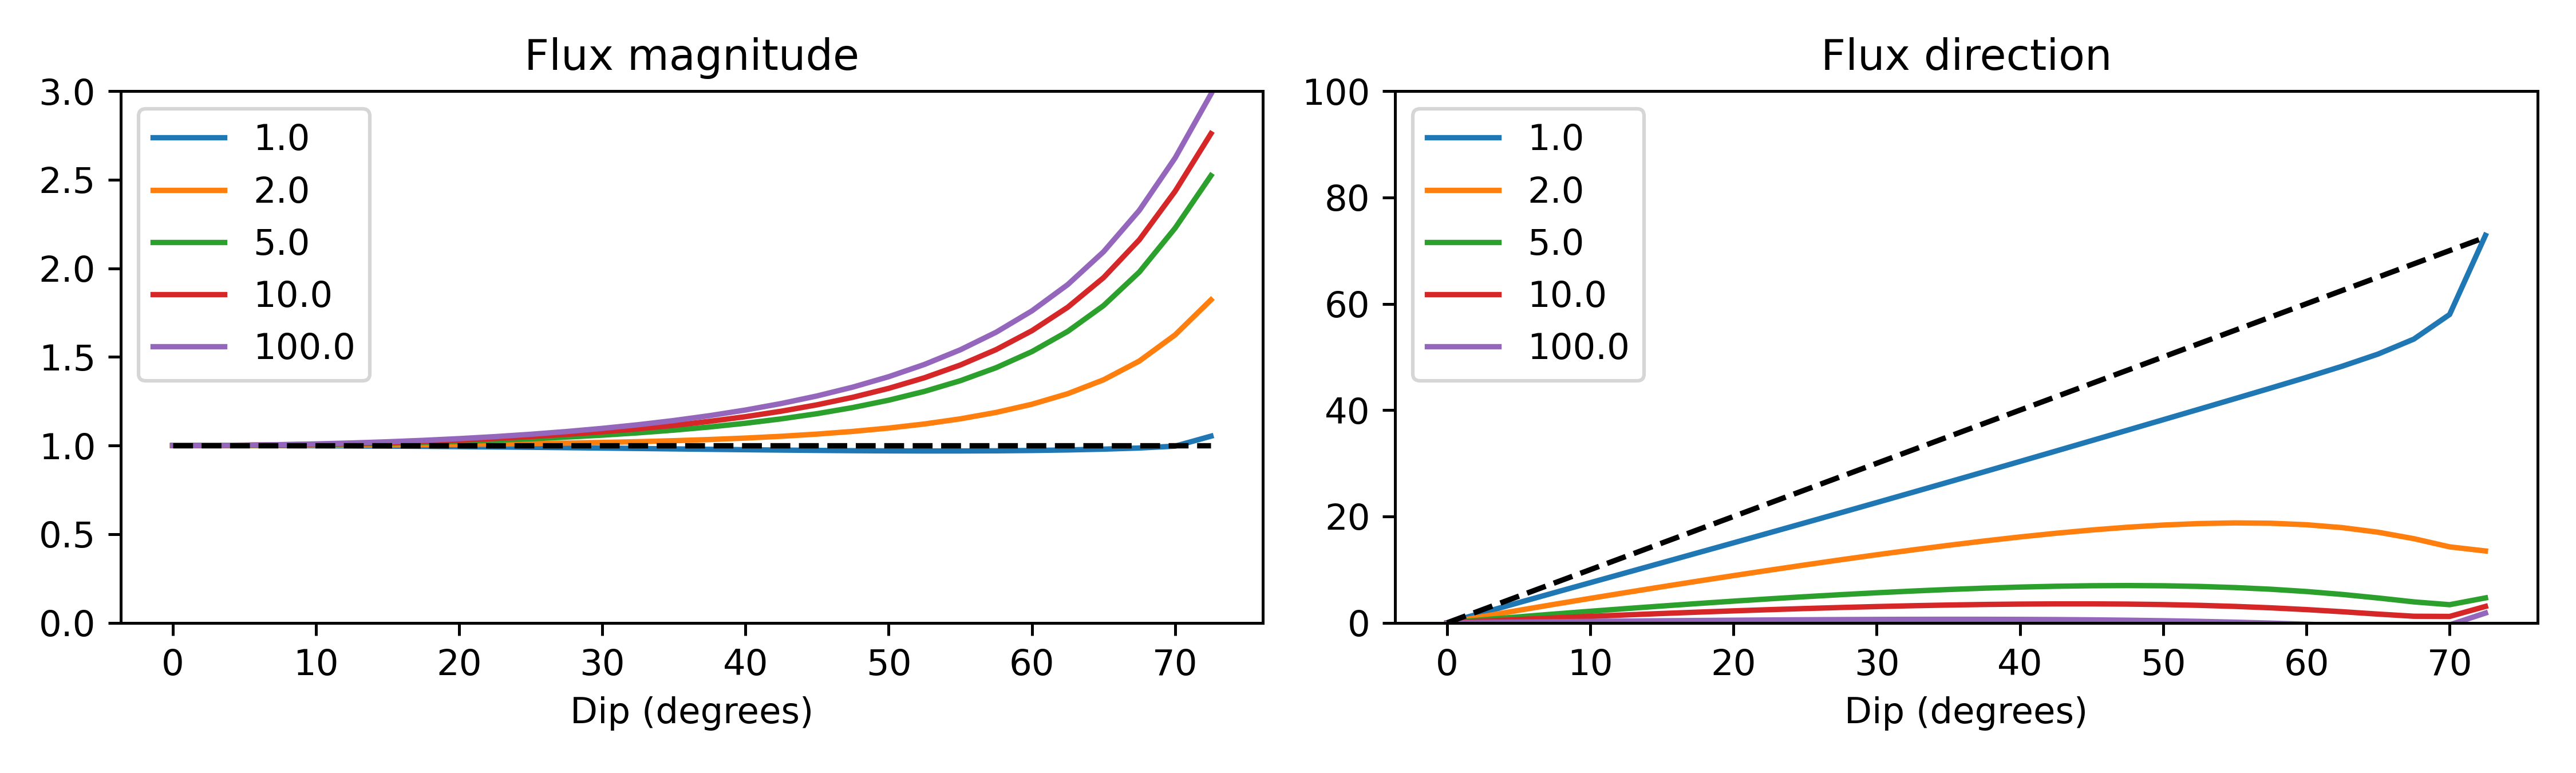
\includegraphics[width=\textwidth]{../figures/fig4_1_paper.png}
%	\caption{layered-connectivity grid, XT3D}
%	\label{fig:fig4b}
\end{subfigure}
\begin{subfigure}{0.9\textwidth}
	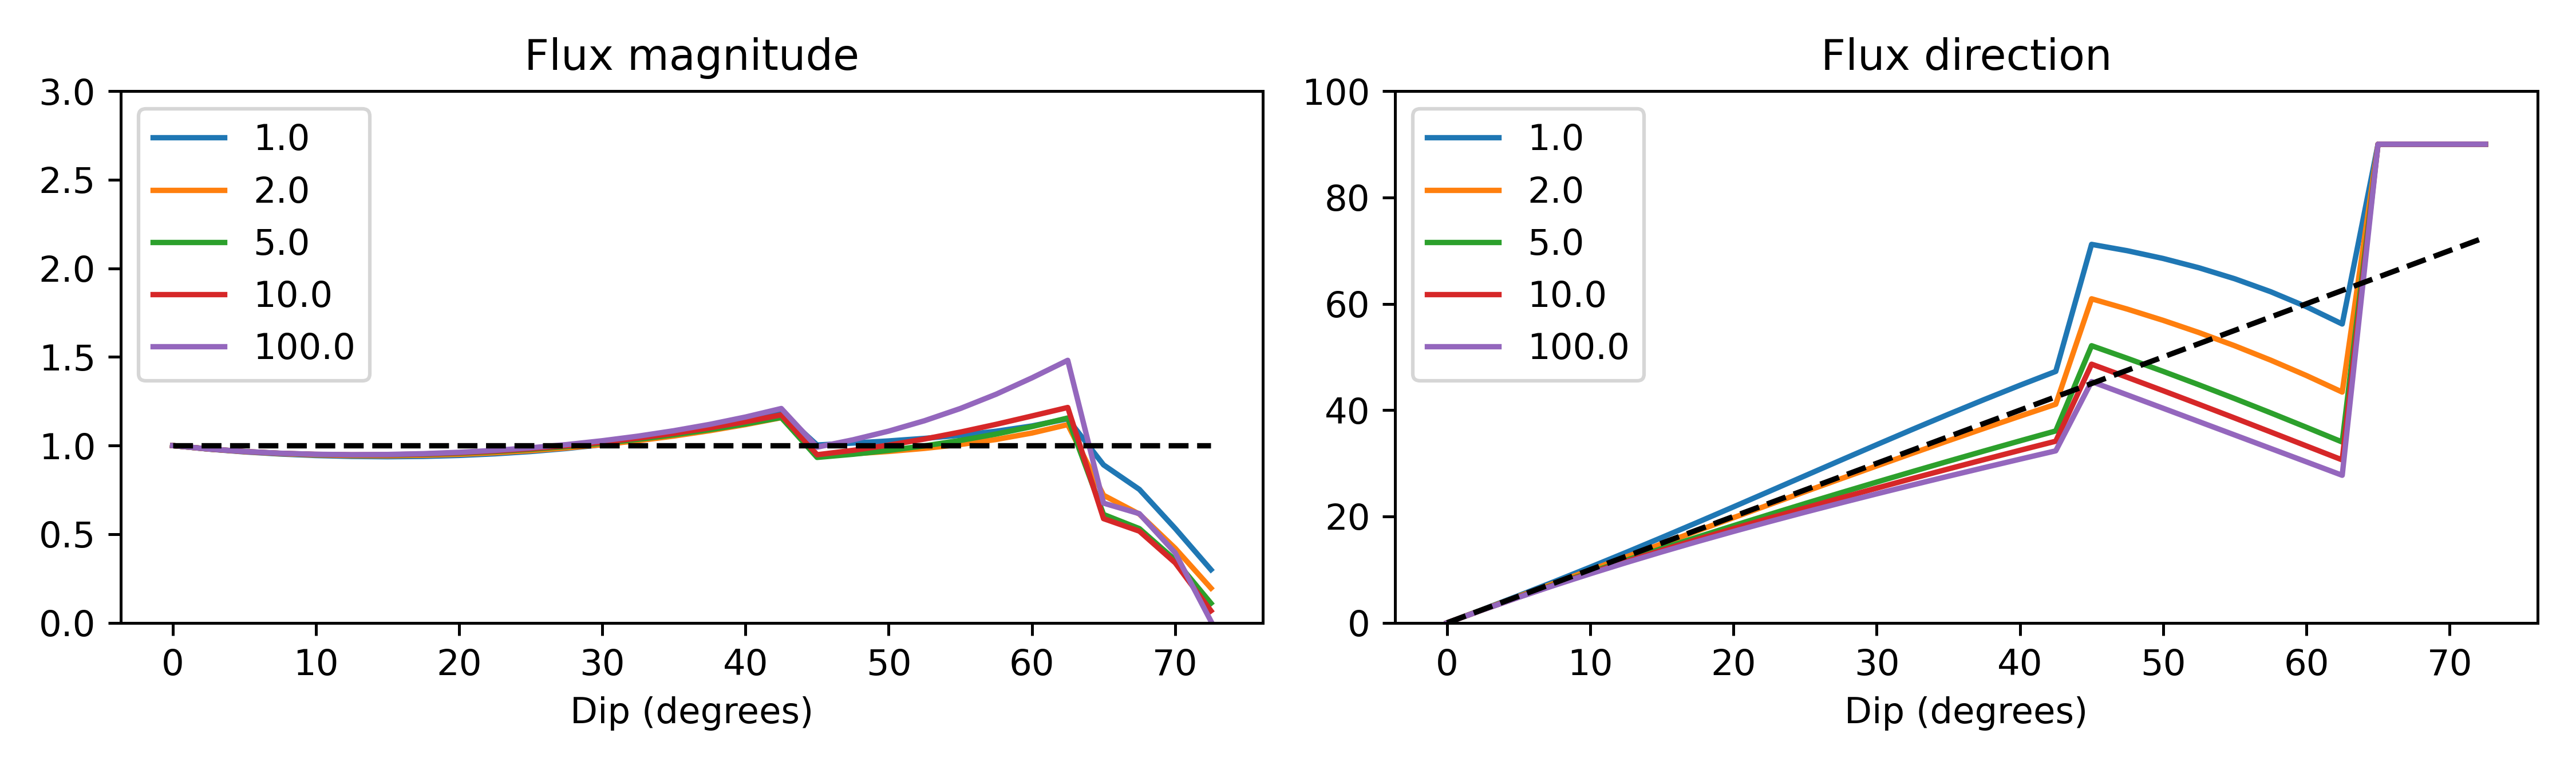
\includegraphics[width=\textwidth]{../figures/fig4_2_paper.png}
%	\caption{full-connectivity grid, standard conductance-based formulation}
%	\label{fig:fig4c}
\end{subfigure}
\begin{subfigure}{0.9\textwidth}
	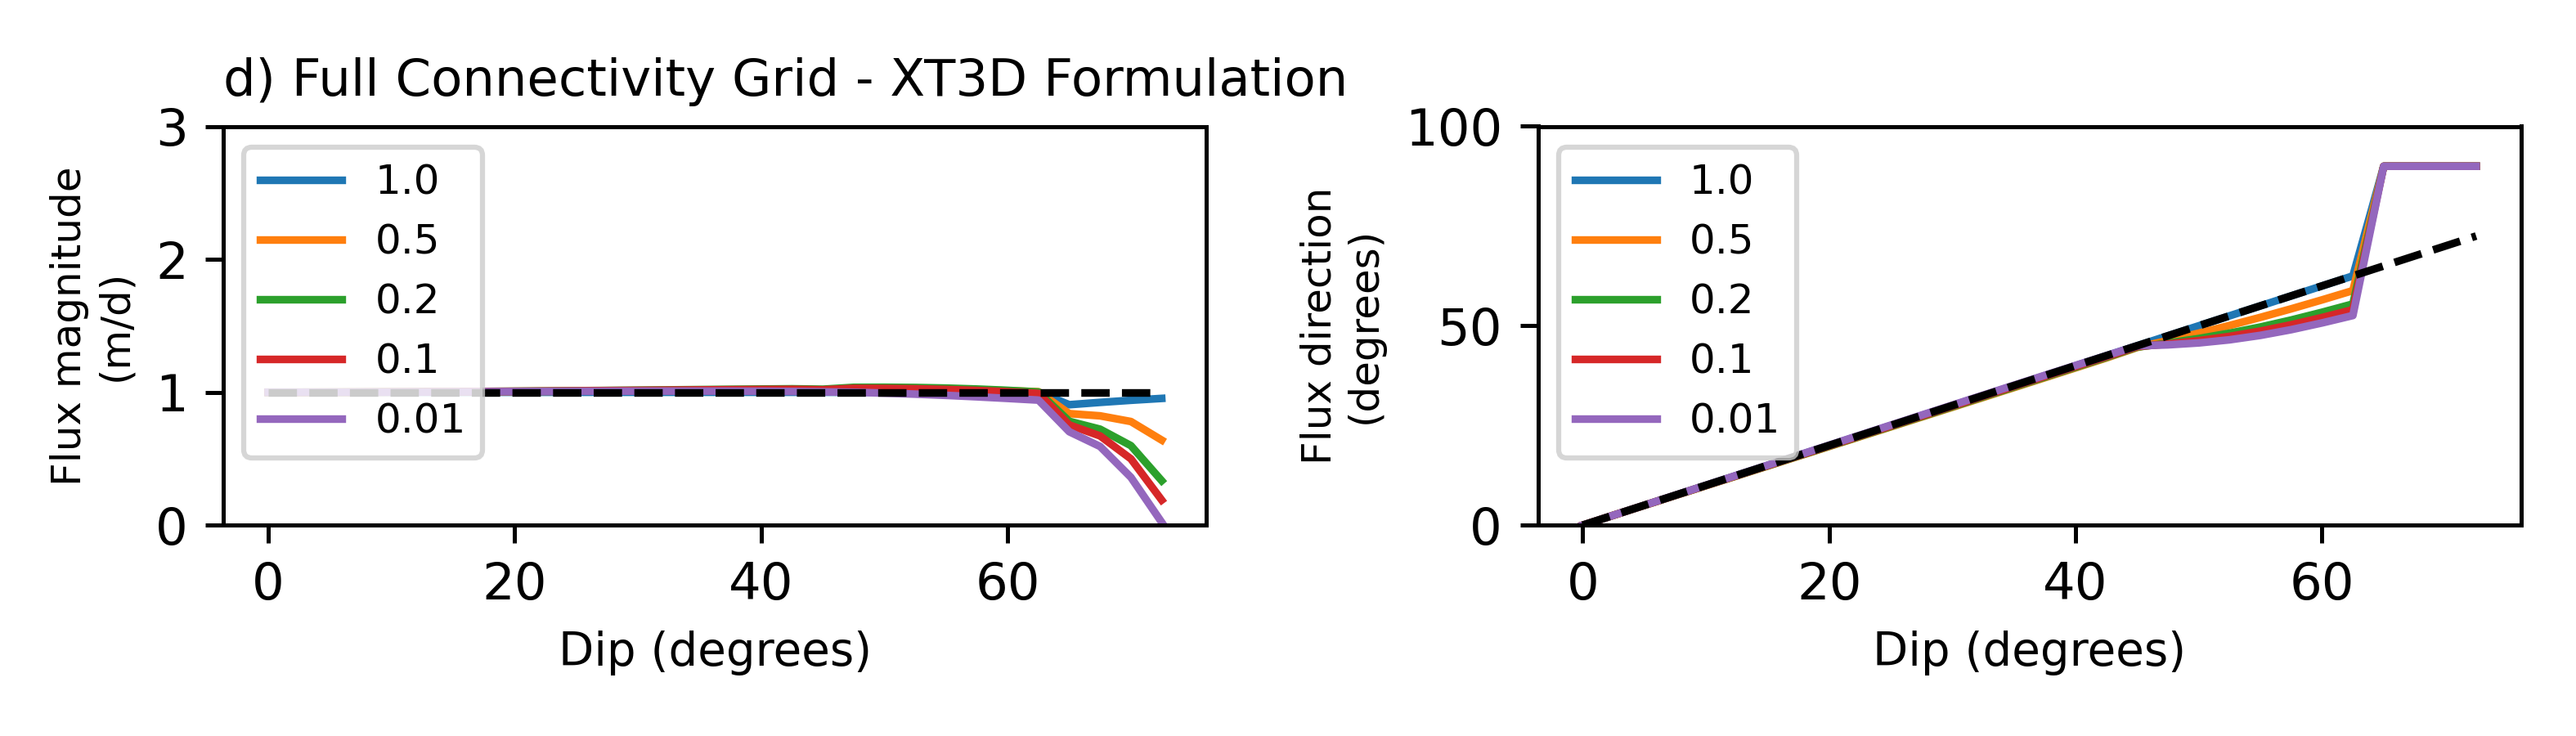
\includegraphics[width=\textwidth]{../figures/fig4_3_paper.png}
%	\caption{full-connectivity grid, XT3D}
%	\label{fig:fig4d}
\end{subfigure}

\caption{Flux magnitude and direction at the cell in the center of the aquifer as a function of aquifer dip angle for various ratios of domain to aquifer conductivity (solid and dash-dotted lines of varying color). The analytical solution is shown as a dashed black line.}
\label{fig:fig4}
\end{figure}

\subsection*{Effect of Anisotropy}

The base case and variations on the base case up to this point have used isotropic hydraulic conductivity. However, sedimentary layers often exhibit anisotropic conductivity. Therefore, we examine the effect of anisotropy within the aquifer and domain by dividing the original conductivity perpendicular to the dip of the aquifer by factors of 1, 10, 100, 1,000 and 10,000 to give anisotropy ratios ranging from 1.0 (isotropic) to 0.0001. Orientation of the principal directions of anisotropy parallel and perpendicular to the dip of the aquifer is accomplished by setting three angles in the NPF Package input. The first angle is the rotation within the horizontal plane of the first principal direction (typically the direction of maximum hydraulic conductivity) with respect to the positive $x$ axis. The second angle is the rotation of the first principal direction upward from the horizontal plane. The third angle is a rotation of the second and third principal directions about the axis of the first principal direction. For this two-dimensional, cross-sectional problem, the first and third angles are set to zero because they represent three-dimensional effects, and the second angle is set equal to the dip angle ($30^{\circ}$).

Layered-connectivity grids produce results that deviate substantially from the analytical solution both with and without the XT3D formulation (Figure \ref{fig:fig5}a), whereas full-connectivity grids with XT3D reproduce the analytical solution (Figure \ref{fig:fig5}b). For example, at an anisotropy ratio of 0.01, use of layered connnectivity produces flow errors of approximately -96\% for both the standard and XT3D flow formulations. Use of full connectivity produces errors of approximately 30\% and -3\% for the standard and XT3D flow formulations, respectively. These results suggest that use of full grid connectivity and the XT3D flow formulation in MODFLOW 6 simulations can be particularly important in the presence of anisotropy.

\begin{figure}
	\begin{center}
	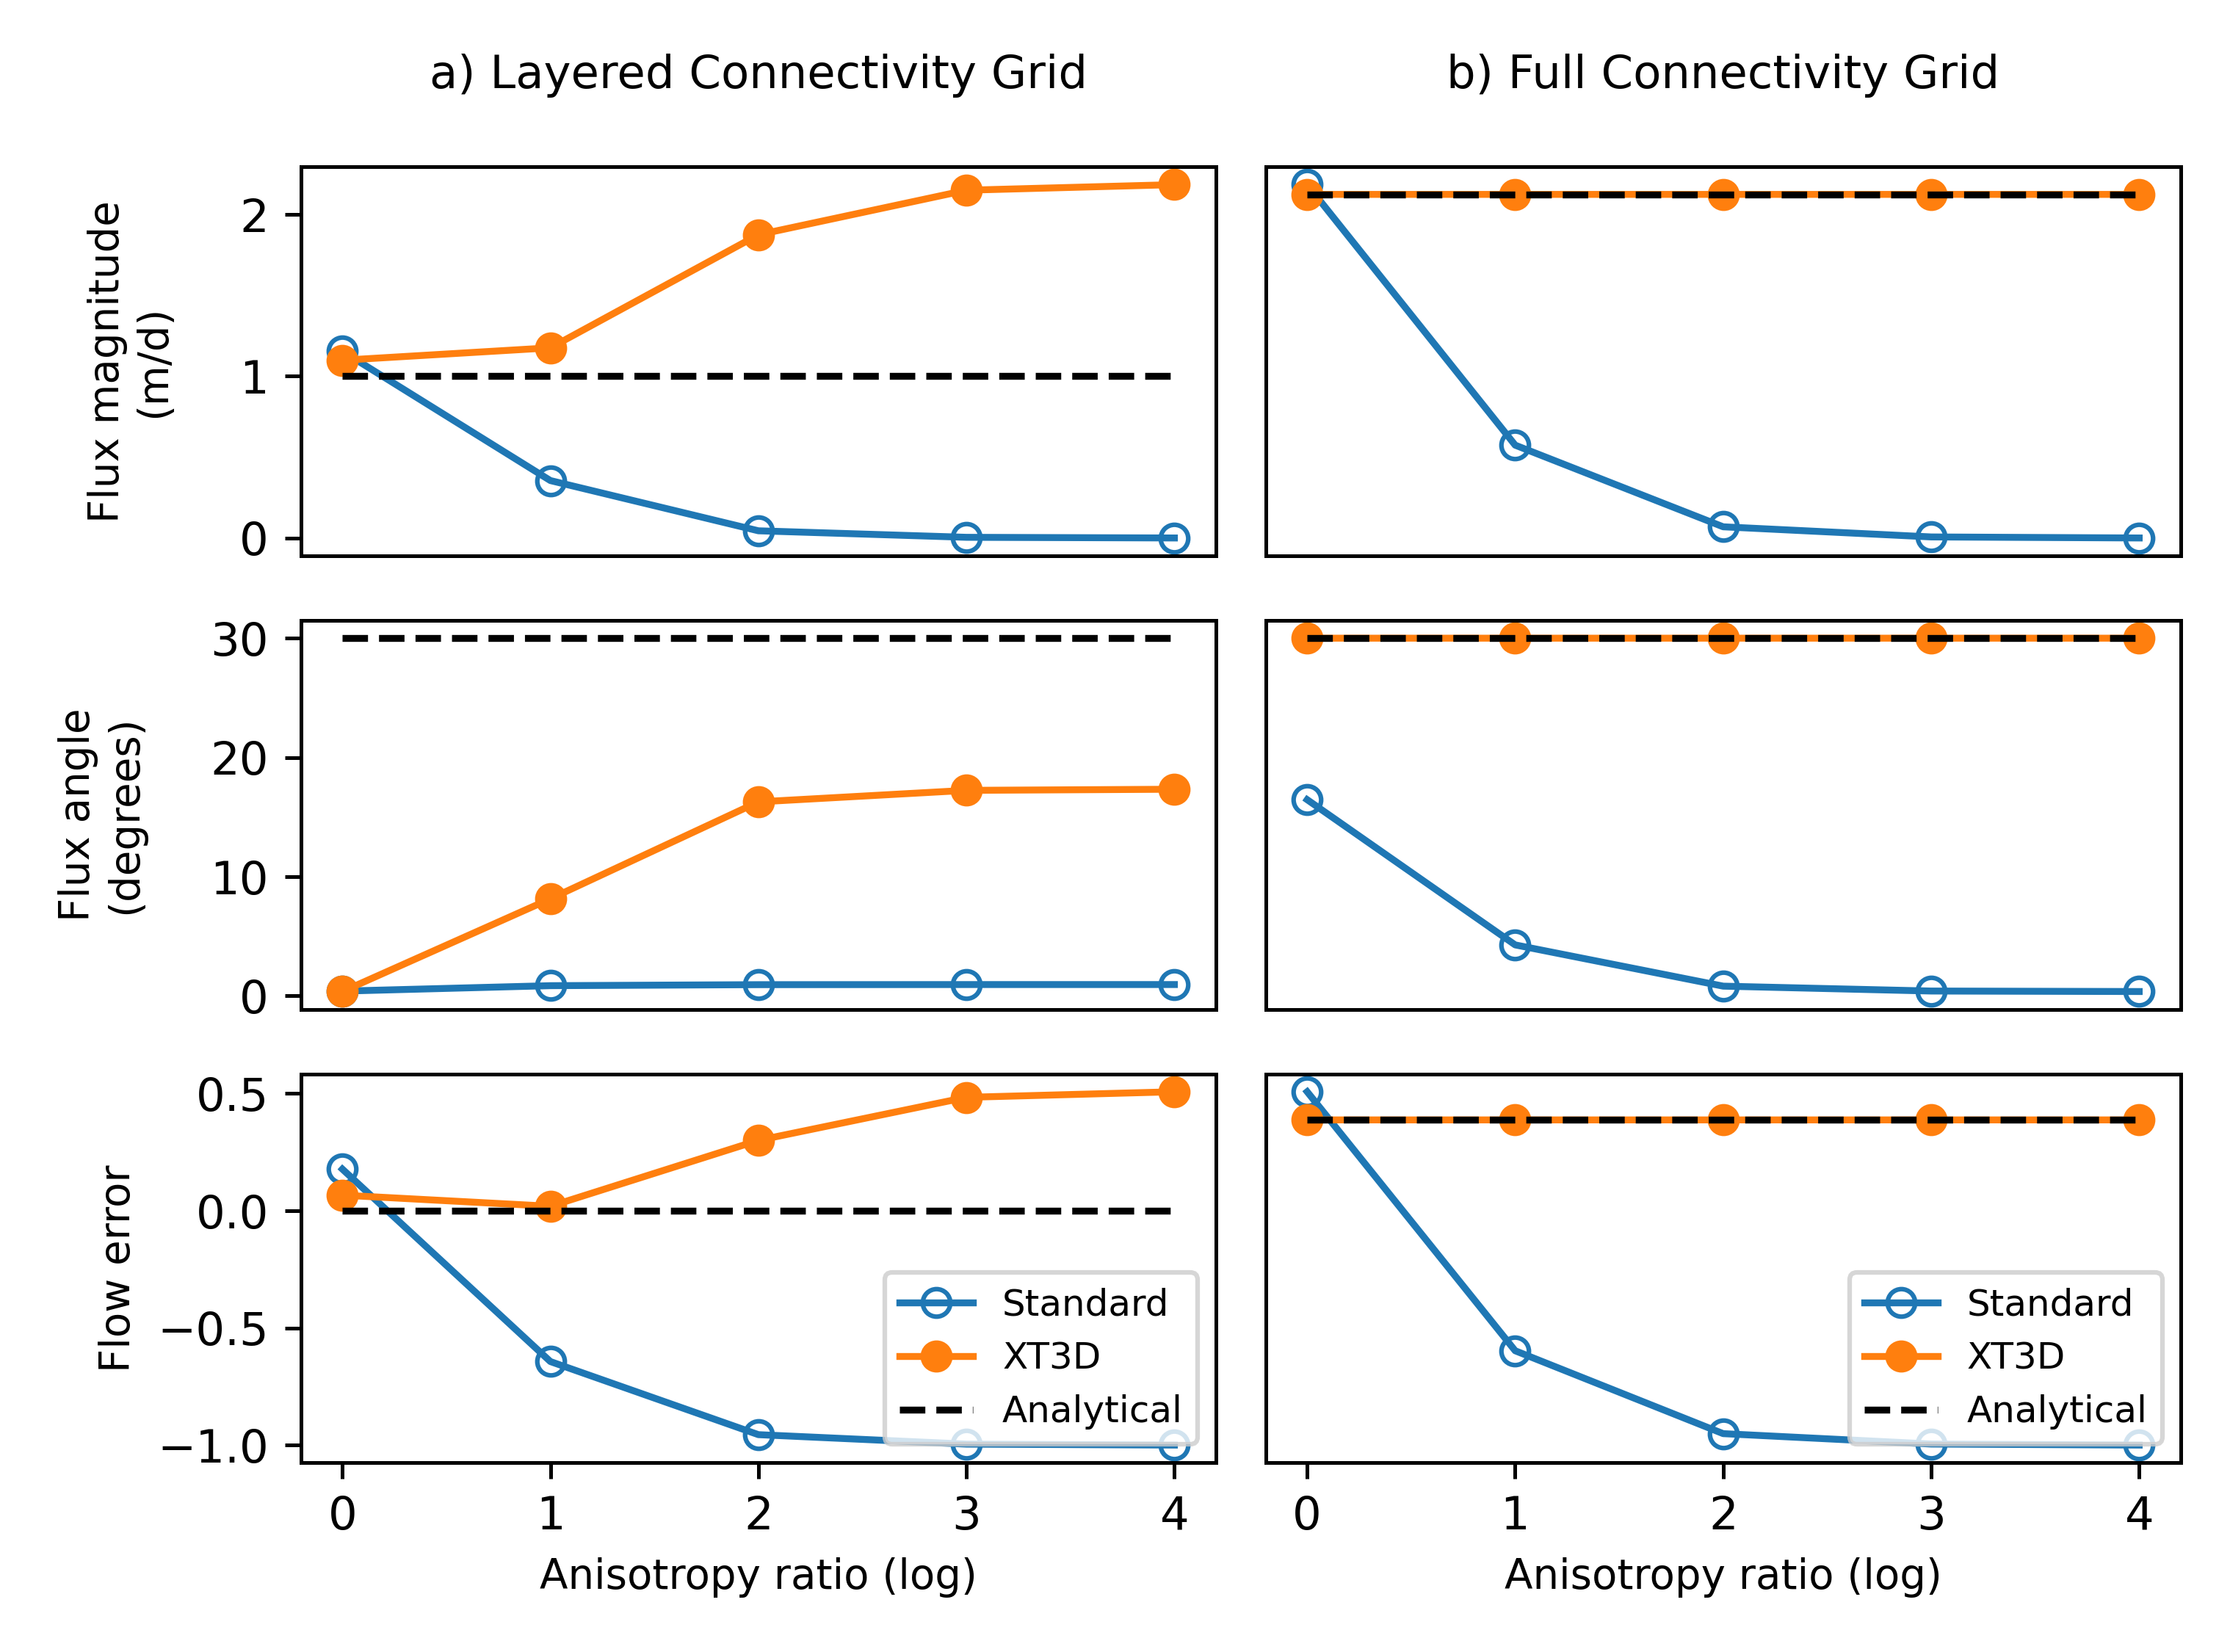
\includegraphics[scale=0.9]{../figures/fig5_paper.png}
	\caption{Graphs indicating how the anisotropy ratio within the aquifer and domain affects the flux magnitude in the center cell (top), the flux direction in center cell (middle) and the volumetric flow through the aquifer (bottom). Errors are minimized by using full connectivity (right column) and the XT3D flow formulation (orange lines with solid circles).}
	\label{fig:fig5}
	\end{center}
\end{figure}

\section*{Conclusions}

\cite{bardot2023} revisited the capability of MODFLOW 6 to accurately simulate groundwater flow through sedimentary structures. They observed that calculated flows involved substantial error in a benchmark problem that simulated flow through a steeply dipping hydrogeologic layer using vertically offset grids, whether or not the XT3D multi-point flow formulation was used. They hypothesized that inadequate lateral connectivity between model cells was responsible for the inability to obtain accurate flow results in their benchmark problem.

In this paper, we have confirmed that the layered lateral connectivity offered by DIS and DISV model grids can be inadequate for simulating groundwater flow through steeply dipping sedimentary structures, even when the XT3D multi-point flow formulation is used.  However, when connections between laterally adjacent cells in different grid layers are added using the fully unstructured (DISU) grid type to comprise a grid with full connectivity, the accuracy of simulated flows can increase substantially. This accuracy improvement requires that at least two grid layers be used to represent the dipping aquifers, with additional grid layers required for very steep dips.

Note that vertical offsets could be avoided when modeling a 2D cross-section using MODFLOW 6 by formulating the model in plan view, such that rows of neighboring cells play the role of model layers. This would allow a DISV grid to follow the top and bottom surfaces of a sloping aquifer in a piecewise-linear fashion without vertical offsets. For a 3D model, an alternative could be to use a simulator based on the finite element method \citep[see, e.g.,][]{yager2009anisotropy}. In evaluating any alternative approach, the ability to accurately simulate flows on the resulting grid, possibly in the presence of anisotropy that is not aligned with the grid, remains one of the considerations.

Our benchmark results suggest that, given appropriate discretization and cell connectivity, the XT3D multi-point flow formulation implemented in MODFLOW 6 can be combined with vertically offset grids to efficiently and accurately simulate flows through steeply dipping sedimentary structures. Our benchmark problem, which is patterned after that of \cite{bardot2023}, features a two-dimensional cross-section with flow along a dipping aquifer of uniform thickness that is discretized using square model cells. Additional investigation is needed to assess the accuracy of calculated flows under different hydraulic gradients and more typical cell aspect ratios, and to better understand the implications of grid connectivity for more complex and realistic flow systems.

The importance of adequate grid connectivity has been explained and demonstrated in this work specifically in terms of hydrogeologic layers that correspond to sedimentary structures. However, the effect of cell connectivity on the accuracy of simulated flows could be important in any MODFLOW application that simulates flow through a heterogeneous hydraulic conductivity field using a grid with large vertical offsets between laterally adjacent cells, whether or not the grid has an explicitly layered structure. 

Our idealized benchmark problem serves as a reminder of the assumptions and limitations inherent in the use of vertically offset grids and points to conditions under which full cell connectivity might be of benefit in practical modeling studies. When such conditions exist in a MODFLOW 6 model, investigation of the effect of cell connectivity may be warranted. In a complex, real-world model, uncertainty in the structure and properties of hydrogeologic units, stresses on the system, and other model parameters could lead to compensation for the effects of inadequate cell connectivity during model calibration. However, when unrealistic flows or parameter values are observed in a calibrated model, inadequate cell connectivity can be considered among the possible sources of structural error, and full connectivity can be considered as a remedy.

\section*{Acknowledgments}
Kerry Bardot is supported by The Australian Research Council, The Western Australian Department of Water and Environmental Regulation and The Water Corporation of Western Australia through grant number LP18101153. The authors sincerely thank James Rumbaugh, John Masterson, Kalle Jahn, Jacob LaFontaine, John Brakebill, Heather Welch, Randall Hunt, and Richard Yager for their review comments, which improved the clarity of the manuscript and refined our conclusions regarding the practical implications of this study. Any use of trade, firm, or product names is for descriptive purposes only and does not imply endorsement by the U.S. Government.

\section*{Supporting Information}
The files that support the creation and running of the test problem are available at https://doi.org/10.5066/P13BNARA.

\bibliography{references.bib}


\end{document}
